\chapter{Relações}

Relações entre elementos de conjuntos ocorrem em muitos contextos. Todos dias lidamos com relações como por 
exemplo: uma pessoa e o seu número de telemóvel, um empregado(a) e o seu salário, etc. Em matemática estudamos
relações como as que existem entre um número inteiro positivo e um seu divisor, um inteiro e o seu quadrado, um 
valor real $x$ e o valor $f(x)$ onde $f$ é uma função, etc.

As relações são representadas utilizando uma estrutura chamada de \emph{relação}, que é simplesmente um subconjunto
do produto cartesiano de conjuntos. As relações podem ser utilizadas para resolver problemas tais como: determinar quais
pares de cidade estão ligadas pela mesma companhia área numa rede, armazenamento de informações em bases de dados, etc.

\section{Relações e suas propriedades}


A forma mais directa de expressar uma relação entre elemento de dois conjuntos é por utilizar pares ordenados (dois elementos).
Por esta razão, os conjuntos de pares ordenados são chamados de \emph{relações binárias}. Nesta secção apresentamos
a terminologia básica utilizada para descrever as relações binárias.

\begin{description}
	\item[Definição 1] Sejam $A$ e $B$ conjuntos, uma relação binária de $A$ para $B$ é um subconjunto de $A \times B$
\end{description}

Por outras palavras uma relação binária de $A$ para $B$ é um conjunto $R$ de pares ordenados onde o primeiro elemento
de cada par ordenado provem de $A$ e o segundo elemento provem de $B$. Utilizamos a notação $a R b$ para denotar 
que $(a,b) \in R$ e $a \not{R} b$ para denotar que $(a,b) \notin R$. Além disso, quando $(a,b)$ pertecem a $R$, dizemos
que $a$ \emph{está relacionado} a $b$ por intermédio de $R$.

As relações binárias representam relacionamentos entre elementos de dois conjuntos. Apresentaremos mais adiante 
as relações n-árias que expressam relacionamentos entre elementos de mais de dois conjuntos. Iremos omitir a palavra
\emph{binária} sempre que não houver perigo de má interpretação. Os exemplos a seguir ilustram o conceito de \emph{relação}.

\begin{description}
	\item[Exemplo 1] {Sejam $A$ o conjunto dos estudantes da tua escola, e $B$ o conjunto das disciplinas. Seja $R$ a 
	a relação que consite nos pares $(a,b)$, onde $a$ é um estudante inscrito na disciplina $b$. Por exemplo, se João e David
	estão inscritos na disciplina de Estruturas Discretas (ED), os pares (João, ED) e (David, ED) pertecem a $R$. Note que
	se David não está inscrito na disciplina de ED, então o par (David, ED) não pertence a $R$. Se um estudante
	não está inscrito em nenhuma disciplina, não existirá nenhum par em $R$ com este estudante como primeiro elemento. Da
	mesma forma se uma disciplina não existe não existirá nenhum par em $R$ com esta discplina como segundo elemento.}
\end{description}

\begin{description}
	\item[Exemplo 2] {Sejam  $A = \{0,1,2\}$ e $B = \{a,b\},$ então $\{(0,a), (0,b), (1,a), (2,b)\}$ é uma relação
	de $A$ para $B$. Isto significa que, por exemplo, $0 R a$, mas $1 \not{R} b$.}. Continua
\end{description}

\section{Relações n-árias}

%Aula de quarta feira
\section{Representação de relações}

\subsection{Introdução}

\textbf{Nota}: Nesta secção, utilizaremos sómente as relações binárias. Por esta razão a palavra relação irá apenas referir-se a
relações bináris. 

Existem muitas formas de representar uma relação entre conjuntos finitos. Uma forma é por listar os pares ordenados.
Outra forma de representar uma relação é por meio de tabelas como vimos na secção anterior. Nesta secção vamos apresentar
dois métodos de representação alternativos: matrizes zero-um e gráfos direccionados. No geral, as matrizes são apropriadas
para a representação de relações em programas de computador. Por outro lado, algumas pessoas acham a representação
de relações utilizando grafos direcconados mais útil ao entendimento das propriedades dessas relações.

\subsection{Representação de relações por meio de matrizes}

A relação entre conjuntos finitos pode ser representada utilizando matrizes zero-um. Suponha que $R$ é uma relação
de $A = \{a_1, a_2, \ldots, a_m\}$ para $B = \{b_1, b_2, \ldots, b_n\}$. (Aqui os elementos dos conjuntos A e B são listados
duma forma particular, embora arbitrária. Além dos maais, quando $A = B$ utilizamos a mesma ordenação para $A$ e $B$.)
A relação $R$ pode ser representada pela matriz $M_R = [m_{ij}]$,\\


$m_{ij} = \begin{cases}
	1$ se $(a_i, b_j) & \in R,\\
	0$ se $(a_i, b_j) & \notin R.
\end{cases}$


Por outras palavras, a matriz zero-um que representa $R$ tem o valor 1 em $(i,j)$ quando $a_i$ está relacionado
a $b_j$, e o valor 0 nesta posição se $a_i$ não está relacionado a $b_j$. Esta representação depende da ordem utilizada
para $A$ e $B$. A utilização de matrizes para representar relações é ilustrados no exemplos a seguir.

\begin{description}
	\item[Exemplo 1] {Suponha que $A = \{1,2,3\}$ e $B = \{1,2\}$. Seja R a relação de $A$ para $B$ contendo os pares
	$(a,b)$ se $a \in A$, $b \in B$ e $a > b$. Qual é matriz que representa $R$ se $a_1 = 1$, $a_2 = 2$, $a_3 = 3$ e 
	$b_1 = 1$ e $b_2 = 2?$}
\end{description}

\emph{Solução:} Como $R = \{(2, 1), (3, 1), (3, 2)\}$, a matriz para $R$ é:

\[
M_R = \begin{bmatrix}
	0 & 0\\
	1 & 0\\
	1 & 1
\end{bmatrix}
\]

Os 1s em $M_R$ mostram que os pares $(2,1), (3,1)$ e $(3,2)$ pertencem a $R$. Os 0s mostram que os outros pares não
pertencem a $R$.

\begin{description}
	\item[Exemplo 2]{Sejam $A = \{a_1, a_2, a_3\}$ e $B = \{b_1, b_2, b_3, b_4, b_5\}$, quais pares ordenados estão na
	relação $R$ representada pela matriz}
\end{description}

\[
	M_R = \begin{bmatrix}
	0 & 1 & 0 & 0 & 0\\
	1 & 0 & 1 & 1 & 0\\
	1 & 0 & 1 & 0 & 1
	\end{bmatrix}?
\]
	
\emph{Solução} Como $R$ consiste nos pares ordenados $(a_i, b_j)$ com $m_{ij} = 1$ daí resulta que
$R = \{(a_1,b_2), (a_2,b_1), (a2, b3), (a2, b4), (a3, b1), (a3, b3), (a3, b5)\}$

A matriz de uma relação em um conjunto, que é uma matriz quadrada, pode ser utilizada para determinar se a relação
possui certas propriedades. Sabemos que uma relação $R$ num conjunto $A$ é reflexiva se $(a,a) \in R$ sempre que
$a \in A$, então, $R$ é reflexiva se e somente se $(a_i, a_i) \in R$ para $i = 1,2,\ldots,n$. Assim, $R$ é reflexiva
se e somente se $m_{ii} = 1$, para $i = 1,2,\ldots,n$. Por outras palavras, $R$ é reflexiva se todos os elementos
da diagonal principal de $M_R$ são iguais a $1$, como ilustrado na Figura \ref{Figura61}. Note que os elementos fora da diagonal
podem ser $0s$ ou $1s$.

\begin{figure}[H]
	\centering
	\[
	\begin{bmatrix}
	 1	& 	& 	&	&	&	&	&\\
	 	& 1 &	&	&	&	&	&\\
		&	& 1 &	&	&	&	&\\
		&	&  	& .	&	&	&	&\\
		&	&	& 	& . &	&	&\\
		&	&	&	&	& . &	&\\
		&	&	& 	&	&	& 1	&\\
		&	&	&	&	&	&	& 1 
	\end{bmatrix}
	\]
	\caption{A matriz zero-um para uma relação reflexiva. (Os elementos fora da diagonal podem ser 0 ou 1.)}
	\label{Figura61}
\end{figure}

A relação $R$ é simétrica se $(a,b) \in R$ implica que $(b, a) \in R$. Consequentemente, a relação $R$ no conjunto
$A = \{a_1, a_2, \ldots, a_n\}$ é simétrica se e somente se $(a_j, a_i) \in R$ sempre que $(a_i, a_j) \in R$. Em termos
dos valores de $M_R$, $R$ é simétrica se e somente se $m_{ji} = 1$ sempre que $m_{ij} = 1$. Isto também significa que 
$m_{ji} = 0$ sempre que $m_{ij} = 0$. Consequentemente, $R$ é simétrica se e somente se $m_{ij} = m_{ji}$, para todos
os pares de inteiros $i$ e $j$ com $i = 1,2,\ldots,n$ e $j=1,2,\ldots,n$. $R$ é simétrica se e somente se $M_R = (M_R)^t$
onde $(M_R)^t$ é matriz transposta de $M_R$.


A relação $R$ é antissimétrica se e somente se $(a, b) \in R$ e $(b, a) \in R$ implica que $a = b$. Consequentemente,
a matrix de uma relação antissimétrica tem a propriedade de que se $m_{ij} = 1$ com $i \ne j$, então $m_{ji} = 0$.
Ou, em outras palavras, $m_{ij} =0$ ou $m_{ji} =0$ quando $i \ne j$. A forma da matriz para uma relação antissimétrica
é ilustrada na Figura \ref{Figura62}.

\begin{figure}[H]
	\centering
	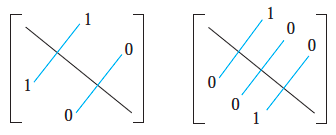
\includegraphics[scale=0.75]{aulas/imagens/62}
	\caption{A matriz zero-um para uma relação simétrica e antissimétrica.}
	\label{Figura62}
\end{figure}

Suppose that the relation R on a set is represented by the matrix

\begin{description}
	\item[Exemplo 3]{Suponha que a relação $R$ é representada pela matriz}
\end{description}
\[
	M_R = \begin{bmatrix}
	1 & 1 & 0\\
	1 & 1 & 1\\
	0 & 1 & 1
	\end{bmatrix}?
\]

$R$ é reflexiva, simétrica e/ou antisimétrica?

\emph{Solução:} Como todas os elementos das diagonais nesta matriz são iguais a $1$, $R$ é reflexiva.
Além do mais, como $M_R$ é simétrica, então $R$ é simétrica. É também fácil notar que $R$ não é antissimétrica.


As operações booleanas estudados anteriormente também podem ser utilizados para encontrar as matrizes que 
representam a união e a intersecção de duas relações. Suponha que $R_1$ e $R_2$ são relações num conjunto $A$
representada pelas matrizes $M_{R_1}$ e $M_{R_2}$, respectivamente. A matriz que representa a união destas duas
relações possui o valor $1$ nas posições em que  $M_{R_1}$ ou $M_{R_2}$ possuem o valor $1$. A matriz que representa a
intersecção destas duas relações possui o valor $1$ nas posições em que  $M_{R_1}$ e $M_{R_2}$ possuem o valor $1$.
Sendo assim, as matrizes que representam a união e a intersecção destas duas relações são

$M_{R_1 \cup R_2} = M_{R_1} \lor M_{R_2}$ e $M_{R_1 \cap R_2} = M_{R_1} \land M_{R_2}$

\subsection{Representação de relações por meio de grafos direccionados}

Vimos anteriormente que uma relação pode ser representada por uma listagem de todos os seus pares ordenados ou por meio
de uma matriz zero-um. Existe outra forma importante de representar uma relação utilizando uma representação 
pictural. Cada elemente do conjunto é representado por um ponto, e cada par ordenado é representado utilizando um arco
cuja direcção indicada por uma seta. Utilizamos essa representação sempre que utilizamos uma relação num conjunto finito como
um grafo direccionado ou dígrafos.


\begin{description}
	\item[Definição 1]{Um \emph{grafo direccionado}, ou \emph{dígrafo}, consiste num conjunto $V$ de \emph{vértices} 
	(ou \emph{nós}) e um conjunto $E$ pares ordenados dos elementos de $V$ chamados de \emph{arestas} (ou \emph{arcos}). 
	O vértice $a$ é chamado de \emph{vértice inicial} da aresta $(a,b)$, e o vértice $b$ é chamado de \emph{vértice terminal}
	desta aresta.}
\end{description}

Uma aresta da forma $(a, a)$ é representada utilizando um arco do vértice $a$ de volta à sí mesmo. Tal aresta é chamada de 
\textbf{laço} ou \textbf{loop}.


\begin{description}
	\item[Exemplo 4]{O grafo direccionado com os vértices $a, b, c$ e $d$ e as arestas $(a,b), (a,d), (b,b), (b,d), (c,a)
	(c,b)$ e $(d,b) é apresentado na Figura \ref{Figura63}$
	}
\end{description}

\begin{figure}[H]
	\centering
	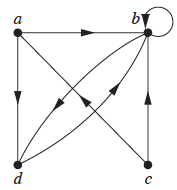
\includegraphics[scale=0.75]{aulas/imagens/63}
	\caption{Um grafo direccionado.}
	\label{Figura63}
\end{figure}


A relação $R$ no conjunto $A$ é representada pelo grafo ordenado que possui elementos de $A$ como seus vértices e os pares 
ordenados $(a,b)$, onde $(a,b) \in R$, como arestas. Esta atribuição configura uma correspondência um-para-um entre as relações
no conjunto $A$ e os grafos direcionados que possuem $A$ como o seu conjunto de vértices. Assim, cada afirmação sobre relações
corresponde a uma afirmação sobre grafos direccionados, e vice-versa. Grafos direccioandos fornecem uma exibição visual das
relações e por isso são utilizados no estudo das relações e de suas propriedades. A utilização de grafos direccionados 
na represetntação de relações num conjunto é ilustrada nos seguintes exemplos.

The directed graph of the relation

on the set {1, 2, 3, 4} is shown in Figure 4.


\begin{description}
	\item[Exemplo 5]{
	O grafo direccionado da relação\\
	$R = {(1, 1), (1, 3), (2, 1), (2, 3), (2, 4), (3, 1), (3, 2), (4, 1)}$\\
	no conjunto ${1, 2, 3, 4}$ é ilustrado na Figura \ref{Figura64}
	}
\end{description}

\begin{figure}[H]
	\centering
	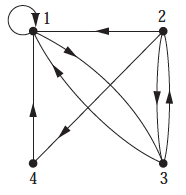
\includegraphics[scale=0.75]{aulas/imagens/64}
	\caption{Um grafo direccionado.}
	\label{Figura64}
\end{figure}

\begin{description}
	\item[Exemplo 6]{
	Quais são os pares ordenados na relação $R$ que representada pelo grafo direccionado da Figura \ref{Figura65}}
\end{description}

\begin{figure}[H]
	\centering
	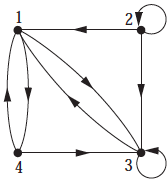
\includegraphics[scale=0.75]{aulas/imagens/65}
	\caption{Um grafo direccionado da relação R.}
	\label{Figura65}
\end{figure}

\emph{Solução:} Os pares ordenados $(x,y)$ na relação na relação são\\
$R = {(1, 3), (1, 4), (2, 1), (2, 2), (2, 3), (3, 1), (3, 3), (4, 1), (4, 3)}$

Cada um destes pares corresponde à uma aresta do grafo direccionado sendo $(2,2)$ e $(3,3)$ dois laços.

O grafo direccionado que representa uma relação pode ser utilizado para determinar se a relação possui certas propriedades.
Por exemplo, a relação é reflexiva se e somente se existe um laço em cada vértice do grafo direccionado, de tal forma que
todos os pares ordenados da forma $(x,x)$ ocorrem na relação. A relação é simétrica se e somente se para cada aresta entre vértices
distintos no digrafo existe uma aresta na direcção oposta, tal que $(y,x)$ existe na relação sempre que $(x,y)$ existe na
relação. Da mesma forma, uma relação é antissimétrica se e somente se não existem duas arestas
em direcções opostas entre vértices distintos. Finalmente, uma relação é transitiva se e somente se sempreque
que existe uma aresta de um vértice $x$ para um vértice $y$ e uma aresta de um vértice $y$ para um vértice $z$, existe uma
aresta de $x$ para $z$ (completando um triângulo onde cada lado é aresta direccionada correctamente).


\begin{description}
	\item[Exemplo 7]{Determine se os grafos direccionados apresentados nas Figuras \ref{Figura66} e \ref{Figura67} são
	reflexivos, simétricos, antissimétricos e/ou transitivos}.
\end{description}

\begin{figure}[H]
	\centering
	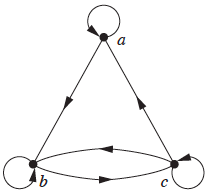
\includegraphics[scale=0.75]{aulas/imagens/66}
	\caption{Um grafo direccionado da relação R.}
	\label{Figura66}
\end{figure}

\begin{figure}[H]
	\centering
	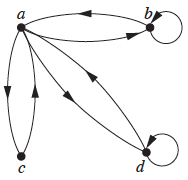
\includegraphics[scale=0.75]{aulas/imagens/67}
	\caption{Um grafo direccionado da relação S.}
	\label{Figura67}
\end{figure}

\emph{Solução:} Como existem laços em todos os vértices do grafo direccionado de $R$, ele é reflexivo. $R$ não é simétrica
nem anti-simétrica porque existe uma aresta de $a$ para $b$ mas não de $b$ para $a$, mas existem arestas em ambas direcções
que conectam $b$ e $c$. Finalmente, $R$ não é transitiva porque existe uma aresta de $a$ para $b$ e uma aresta de $b$ para $c$,
mas não existe uma aresta de $a$ para $c$. Como não existem laços em todo os vértices do grafo direccionado de S, esta relação não é reflexiva. É simétrica
mas não antissimétrica, porque cada aresta entre vértices distintos é acompanhada por uma aresta na direcção oposta. Não é
díficil notar também que o grafo direccionado de $S$ não é transitivo, porque $(c,a)$ e $(a,b)$ pertencem a $S$, mas
$(c,b)$ não pertence a $S$.

Estudaremos os grafos em mais detalhnes no próximo capítulo.


\section{Fechamento de relações}

\subsection{Introdução}

Uma rede de computadores de uma empresa possui centros de dados em Benguela, Bengo, Cabinda, Cunene, Huíla e Luanda.
Existem ligações directas de Benguela para o Bengo, de Benguela para o Bengo, de Benguela para Cunene, do Bengo para o
Cunene, de Cunene para Cabinda e da Huíla para Luanda. Seja $R$ a relação que contém $(a,b)$ se existe uma ligação do 
centro de dados em $a$ com o centro de dados em $b$, como podemos determinar se existe uma ligação (possívelmente indirecta)
composta de uma ou mais linhas de um centro para outro? Como nem todas as ligações são directas, tal como a ligação de
Benguela para Cabinda que passa por Cunene, $R$ não pode ser utilizada directamente para responder esta questão.
Na linguagem das relações, $R$ não é transitiva, portanto não contém todos os pares que podem ser ligado. Tal como iremos
mostrar nesta secção, é possível achar todos os pares de centros de dados que possuem um link por construír
uma relação transitiva $S$ que contém $R$ tal que $S$ é um subconjunto de todas as relações transitivas que contêm $R$.


\section{Relações de equivalência}

\section{Ordens parciais}

\subsection{Exercícios}